\newcommand\tab[1][1cm]{\hspace*{#1}}
\subsection{Uputstvo za repliciranje rezultata}

\begin{enumerate}

\subsubsection{Projektovanje u Quartus-u}
\item U \texttt{Microsoft Windows} operativnom sistemu pokrenuti \texttt{DE1SoC\_SystemBuilder.exe} (dostupan na [])
\item Izabrati konfiguraciju kao na slici \ref{slika:sb} i izabrati Generate\\
\begin{figure}[h!]
\centering
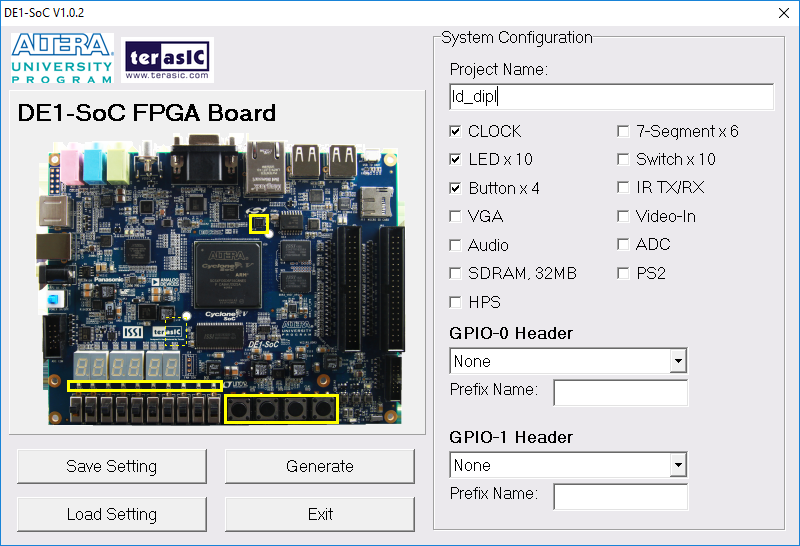
\includegraphics[scale=0.6]{img/DE1SoC_SystemBuilder.png}
\caption{Podešavanja \texttt{DE1\_Soc Bulder}-a}
\label{slika:sb}
\end{figure}
\item  Izbristati \texttt{ld\_dipl.v} fajl (ovaj fajl se ne koristi, kasnije će biti napravljen \texttt{ld\_dipl.vhd} fajl za VHDL)
\item  Kopirati generisane fajlove u \texttt{Ubuntu} u radni folder (u ovom radu je to \texttt{\textasciitilde/ld\_dipl/hw/})
\item  Pokrenuti \texttt{Quartus (Quartus Prime 18.0) Lite Edition}
\item  Otvoriti projekat komandom \texttt{File > Open Project...} i izabrati \texttt{\textasciitilde/ld\_dipl/hw/ld\_dipl.qpf}
\item U prozoru \texttt{Tasks} izabrati \texttt{Edit Settings}, u novom prozoru pod \texttt{Timing Analyser} ispod teksta \texttt{SDC files to include in the project} klikom na dugme '...' izabrati fajl \texttt{ld\_dipl.sdc}
\item  Pokrenuti \texttt{Platform Designer} klikom na \texttt{Tools > Platform Designer}
\item  Iz prozora \texttt{IP Catalog} izabrati \texttt{Processors and Peripherials} \texttt{> Hard Processor Systems >} \texttt{ArriaV/Cyclone V Hard Processor System}. Ovim se otvara meni za podešavanje HPS modula
\item  Pod tabom \texttt{FPGA interfaces} izvršiti sledeće izmene:
\begin{itemize}
\item	U opštim podešavanjima isključiti opciju \texttt{Enable MPU standby and event signals}
\item	U podešavanjima \texttt{AXI Bridges} podesiti \texttt{FPGA-to-HPS interface} i \texttt{HPS-to-FPGA interface} na \texttt{unused}, a \texttt{Lightweight HPS-to-FPGA} na \texttt{32-bit}
\item	U podešavanjima \texttt{FPGA-to-HPS SDRAM Interface} izabrati \texttt{f2h\_sdram0} i zatim isključiti pritiskom na dugme '-'
\item	U podešavanjima \texttt{Interrupts} uključiti opciju \texttt{Enable FPGA-to-HPS interrupts}
\end{itemize}
\item  Pod tabom \texttt{Peripherial Pins} izvršiti sledeće izmene
\begin{itemize}
\item	U podešavanjima \texttt{SD/MMC Controller} postaviti \texttt{SDIO} pin na \texttt{HPS I/O Set 0} i \texttt{SDIO mode} na \texttt{4-bit Data}
\item	U podešavanjima \texttt{UART Controllers} postaviti \texttt{UART0} pin na \texttt{HPS I/O Set 0} i \texttt{UART mode} na \texttt{No Flow Control}
\end{itemize}
	\begin{figure}[h!]
	\centering
	\textit{U ovom tabu je za potrebe nekog drugog projekta moguce uključiti ostale periferije: CAN Controller, Ethernet Media Access Controller, I2C Controller, SPI Controller, QSPI Flash Controller, NAND Flash Controller, Trace Port Intefrace Unit, GPIO za podesavanja pogledati []}
	\end{figure}
\item  Pod tabom \texttt{HPS Clocks} ostaviti podešavanja na podrazumevanim vrednostima
\item  Pod tabom \texttt{SDRAM} podesiti:
\texttt{
\begin{itemize}
\item	SDRAM Protocol: DDR3
\item	PHY Settings:
\begin{itemize}
\item		Clocks:
\begin{itemize}
\item			Memory clock frequency: 400.0 MHz
\item			PLL reference clock frequency: 25.0 MHz
\end{itemize}
\item		Advanced PHY Settings:
\begin{itemize}
\item			Supply Voltage: 1.5V DDR3
\end{itemize}
\end{itemize}
\item	Memory Parameters:
\begin{itemize}
\item		Memory vendor: Other
\item		Memory device speed grade: 800.0 MHz
\item		Total interface width: 32
\item		Number of chip select/depth expansion: 1
\item		Number of clocks: 1
\item		Row address width: 15
\item		Column address width: 10
\item		Bank-address width: 3
\item		Uključiti DM pins
\item		Uključiti \texttt{DQS\#}
\item		Memory Initialization Options:
\begin{itemize}
\item			Mirror Addressing: 1 per chip select: 0
\item			Burst Length: Burst chop 4 or 8 (on the fly)
\item			Read Burst Type: Sequential
\item			DLL precharge power down: DLL off
\item			Memory CAS latency setting: 11
\item			Output drive strength setting: RZQ/7
\item			ODT Rtt nominal value: RZQ/4
\item			Auto selfrefresh method: Manual
\item			Selfrefresh temperature: Normal
\item			Memory write CAS latency setting: 8
\item			Dynamic ODT (\texttt{Rtt\_WR}) value: RZQ/4
\end{itemize}
\end{itemize}
\item	Memory Timing:
\begin{itemize}
\item		tIS (base): 180 ps
\item		tIH (base): 140 ps
\item		tDS (base): 30 ps
\item		tDH (base): 65 ps
\item		tDQSQ: 125 ps
\item		tQH: 0.38 cycles
\item		tDQSCK: 255 ps
\item		tDQSS: 0.25 cycles
\item		tQSH: 0.4 cycles
\item		tDSH: 0.2 cycles
\item		tDSS: 0.2 cycles
\item		tINIT: 500 us
\item		tMRD: 4 cycles
\item		tRAS: 35.0 ns
\item		tRCD: 13.75 ns
\item		tRP: 13.75 ns
\item		tREFI: 7.8 us
\item		tRFC: 260.0 ns
\item		tWR: 15.0 ns
\item		tWTR: 4 cycles
\item		tFAW: 30.0 ns
\item		tRRD: 7.5 ns
\item		tRTP: 7.5 ns
\end{itemize}
\item	Board Settings:
\begin{itemize}
\item		Setup and Hold Derating:
\begin{itemize}
\item			Use Altera's default settings
\end{itemize}
\item		Channel Signal Integrity:
\begin{itemize}
\item			Use Altera's default settings
\end{itemize}
\item		Board Skews:
\begin{itemize}
\item			Maximum CK delay to DIMM/device: 0.03 ns
\item			Maximum DQS delay to DIMM/device: 0.02 ns
\item			Minimum delay difference between CK and DQS: 0.06 ns
\item			Maximum delay difference between CK and DQS: 0.12 ns
\item			Maximum skew within DQS group: 0.01 ns
\item			Maximum skew between DQS groups: 0.06 ns
\item			Average delay difference between DQ and DQS: 0.05 ns
\item			Maximum skew within address and command bus: 0.02 ns
\item			Average delay difference between address and command and CK: 0.01 ns
\end{itemize}
\end{itemize}
\end{itemize}
}
Ovim su podešavanja HPS modula završena, izabrati \texttt{Finish}.
\item  Duplim klikom u \texttt{Export} koloni eksportovati signale \texttt{memory} pod imenom \texttt{hps\_0\_ddr} i signale \texttt{hps\_io} pod imenom \texttt{hps\_0\_io}.
\item  Povezati HPS sa izvorom takta kao što je prikazano na slici \ref{slika:q1}
\begin{figure}[h!]
\centering
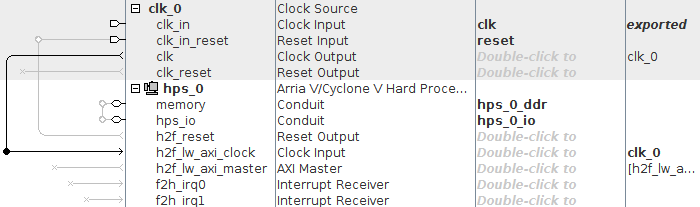
\includegraphics[scale=0.9]{img/quartus1.png}
\caption{Povezivanje HPS i takt signala}
\label{slika:q1}
\end{figure}
\item  Iz prozora \texttt{IP Catalog} izabrati \texttt{Processors and Peripherials > Peripherials > PIO (Parallel I/O) Intel FPGA IP}. Ovim se otvara meni za podešavanje \texttt{PIO IP} bloka
\item  U podešavnjima \texttt{PIO IP} bloka pod \texttt{Basic Settings} postaviti \texttt{Width: 8} i \texttt{Direction: Output}
\item  Preimenovati \texttt{PIO} blok u \texttt{leds\_0}. Duplim klikom u \texttt{Export} koloni eksportovati signale \texttt{external\_connection} i podesiti ime \texttt{leds\_0\_external\_connection}.
\item  Povezati \texttt{leds\_0} blok sa izvorom takta i resetom, zatim povezati Avalon Memory Mapped Slave pod imenom \texttt{s1} sa \texttt{hps\_0} interfejsom \texttt{h2f\_lw\_axi\_master}, kao što je prikazano na slici \ref{slika:q2}
\begin{figure}[h!]
\centering
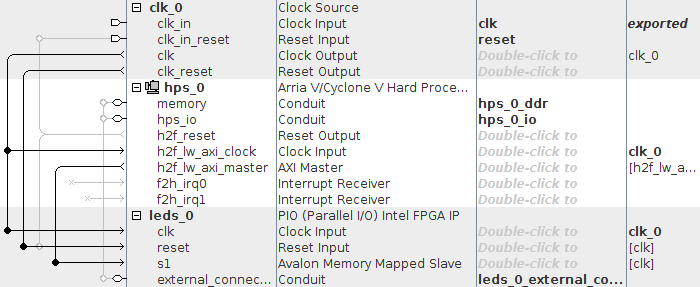
\includegraphics[scale=0.9]{img/quartus2.png}
\caption{Povezivanje \texttt{leds\_0} bloka}
\label{slika:q2}
\end{figure}
\item  Ponovo iz prozora \texttt{IP Catalog} izabrati\texttt{ Processors and Peripherials > Peripherials > PIO (Parallel I/O) Intel FPGA IP}. Ovim se otvara meni za podesavanje \texttt{PIO IP} bloka
\item  U podešavnjima \texttt{PIO IP} bloka pod \texttt{Basic Settings} postaviti \texttt{Width: 8}, \texttt{Direction: Input}.
\item  U podešavanjima \texttt{PIO IP} bloka pod \texttt{Edge capture register} uključiti opciju \texttt{Synchronously capture, Edge Type} podesiti na \texttt{ANY}, i uključiti \texttt{bit-clearing for edge capture register}.
\item  U podešavanjima \texttt{PIO IP} bloka pod \texttt{Interrupt} uključiti opciju \texttt{Generate IRQ} i izabrati \texttt{IRQ Type: EDGE}
\item  Preimenovati \texttt{PIO} blok u \texttt{keys\_0}. Duplim klikom u \texttt{Export} koloni eksportovati signale \texttt{external\_connection} i podesiti ime \texttt{keys\_0\_external\_connection}.
\item  Povezati \texttt{keys\_0} blok sa izvorom takta i resetom, zatim povezati Avalon Memory Mapped Slave pod imenom \texttt{s1} sa \texttt{hps\_0} interfejsom  \texttt{h2f\_lw\_axi\_master} i na kraju povezati \texttt{irq} signal na \texttt{f2h\_irq0} interfejs \texttt{hps\_0} bloka, kao što je prikazano na slici \ref{slika:q3}
\begin{figure}[h!]
\centering
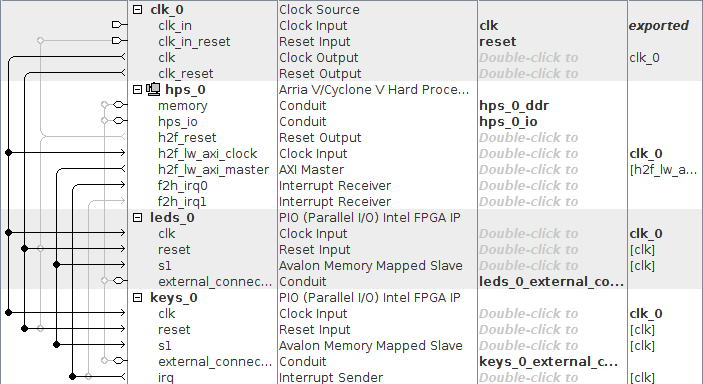
\includegraphics[scale=0.9]{img/quartus3.png}
\caption{Povezivanje \texttt{keys\_0} bloka}
\label{slika:q3}
\end{figure}
\item  Duplim klikom u koloni \texttt{Base} podesiti adresu porta \texttt{s1} bloka \texttt{leds\_0} i porta \texttt{s1} bloka \texttt{keys\_0} kao na tabeli 1.
\item  Sačuvati \texttt{Platform Designer} projekat izborom \texttt{File > Save} i sačuvati ga pod imenom \texttt{ld\_dipl\_system.qsys}
\item  Trebalo bi da se pojavi obaveštenje \texttt{Save System: completed successfully}. Zatim odabrati iz menija \texttt{Generate > Generate HDL... }U novom prozoru podesiti \texttt{Create HDL design files for synthesis: VHDL} i isključiti opciju \texttt{Crete block symbol file (.bsf)}. Pokrenuti generisanje klikom na \texttt{Generate}. Proces bi trebalo da se završi bez grešaka ali može imati upozorenja.
\item  Zatvoriti \texttt{Platform Designer}. U prozoru \texttt{Quartus}-a izabrati \texttt{Project > Add/Remove Files in Project...} i u meniju klikom na '...' izabrati fajl\\ \texttt{ld\_dipl\_system/synthesis/ld\_dipl\_system.qip}.
\item  Izabrati \texttt{File > New VHDL File} i novi fajl nazvati \texttt{ld\_dipl.vhd}. Pod \texttt{Project Navigator > Files} desnim klikom na \texttt{ld\_dipl.vhd} izabrati \texttt{Set as Top-Level Entity}.
\item  U ovom fajlu je potrebno instancirati HPS komponentu iz \texttt{Platform Designer}-a. Potrebno je ručno napiati ovaj fajl (primer za ovaj rad dat je u dodatku. Takođe među generisanim fajovima nalazi se deklaracija komponente \texttt{ld\_dipl\_system} koja može biti od pomoći (fajl \texttt{\textasciitilde/ld\_dipl/hw/ld\_dipl\_system/ld\_dipl\_system.cmp}).
\item  Izabrati \texttt{Processing > Start > Start Analysis and Synthesis}
\item  Izabrati \texttt{Tools > Tcl Scripts...}\\
\begin{figure}[h!]
\centering
\textbf{Važno: Prozor koji se otvori mora da izgleda upravo kao na slici \ref{slika:tcl} (generisani fajlovi ne smeju biti duplirani). Ukoliko su fajlovi duplirani neophodno je zatvoriti \texttt{Quartus} i pokrenuti ponovo. Neke verzije \texttt{Quartus}-a imaju ovu grešku pri detekciji \texttt{tcl} skripti.}\\
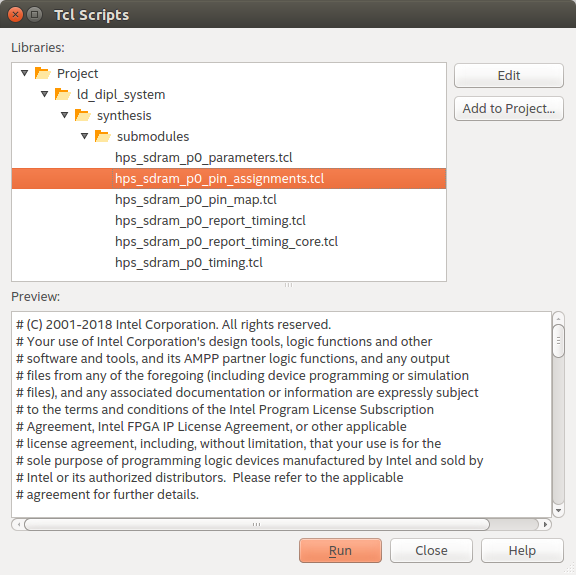
\includegraphics[scale=0.5]{img/tcl.png}
\caption{Ispravan izgled menija}
\label{slika:tcl}
\end{figure}
 
 Izabrati \texttt{hps\_sdram\_p0\_pin\_assignments.tcl} i kliknuti Run. Ukoliko dođe do grešaka proveriti da li je izvršen prethodni korak.
\item  Pokrenuti kompajliranje projekta izborom \texttt{Processing > Start Compilation}

\subsubsection{Podešavanja okruženja i preuzimanje kompajlera}
\item Preuzeti arhivu sa Linaro toolchain-om\\
\texttt{wget https://releases.linaro.org/components/toolchain/binaries/7.2-2017.11/\\arm-linux-gnueabihf/gcc-linaro-7.2.1-2017.11-x86\_64\_arm-linux-gnueabihf.tar.xz}
\item Otpakovati preuzeti toolchain:\\
\texttt{tar -xf arm-linux-gnueabihf/gcc-linaro-7.2.1-2017.11-x86\_64\_arm-linux-gnueabihf.tar.xz \textasciitilde/ld\_dipl/sw/toolchain}
\item Dodati putanju za toolchain u promenljivu okruženja \texttt{PATH}.\\
\texttt{export PATH=\textasciitilde/ld\_dipl/sw/toolchain/bin:\$PATH}
\item Podesiti promenljive okruženja\\
\texttt{export ARCH=arm}\\
\texttt{export CROSS\_COMPILE=arm-linux-gnueabihf-}\\
\item Pokrenuti podešavanja Altera SOC EDS:\\ 
\texttt{cd ~/intelFPGA/18.0/embedded}\\
\texttt{source embedded\_command\_shell.sh}
\item Dodati putanju za Quartus alate u promenljivu okruženja \texttt{PATH}:\\
\texttt{export PATH=\textasciitilde/intelFPGA\_lite/18.0/quartus/bin/:\$PATH}

\subsubsection{Generisanje RBF fajla}
\item \texttt{quartus\_cpf -c -o bitstream\_compression=on \textbackslash \\ \textasciitilde/ld\_dipl/hw/ld\_dipl.sof \textbackslash \\ \textasciitilde/ld\_dipl/sdcard/fat32/socfpga.rbf}
\subsubsection{Generisanje i kompajliranje Preloader-a}
\item Pokrenuti Preloader generator komadnom:\\ \texttt{bsp-editor}
\item Izabrati \texttt{File > New HPS BSP...}
\item U novom prozoru podesiti \texttt{Preloader Settings Directory:} \\ \texttt{ \textasciitilde/ld\_dipl/hw/hps\_isw\_handoff/ld\_dipl\_system\_hps\_0}
\item Isključiti opciju: \texttt{Use default locations} i podesiti \texttt{BSP target directory:} \\ \texttt{\textasciitilde/ld\_dipl/sw/preloader}. Podešavanja bi trebalo da izgledaju kao na slici \ref{slika:bsp1}. Izabrati \texttt{OK}.
\begin{figure}[h!]
\centering
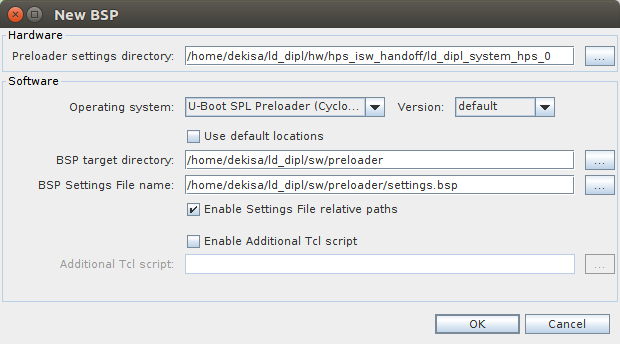
\includegraphics[scale=0.6]{img/bsp1.png}
\caption{Podešavanja \texttt{bsp-editor}-a}
\label{slika:bsp1}
\end{figure}
\item U podešavanjima pod \texttt{spl.boot} uključiti \texttt{FAT\_SUPPORT} i ostala podešavanja ostaviti na podrazumevanim vrednostima. Izabrati \texttt{Generate} i po završenom generisanju zatvoriti program.
\item Izvršiti komande za kompajliranje Preloader-a\\
\texttt{cd \textasciitilde/ld\_dipl/sw/preloader}\\
\texttt{make}
\item Kopirati kompajlirani Preloader:
\texttt{cp \textasciitilde/ld\_dipl/sw/preloader/preloader-mkpimage.bin \textasciitilde/ld\_dipl/sdcard/a2/}\\

\subsubsection{Generisanje Device Tree}
\item Uporebom Alterinog alata generisati \texttt{Device Tree} komandom: \\
\texttt{sopc2dts -i ~/ld\_dipl/hw/ld\_dipl\_system.sopcinfo \\-o ~/ld\_dipl/hw/ld\_dipl\_generated.dts}

\subsubsection{U-Boot}
\item Preuzeti izvorni kod projekta U-boot komandom\\ \texttt{git clone git://git.denx.de/u-boot.git \textasciitilde/ld\_dipl/sw/u-boot}
\item Promeniti radni direktorijum\\ \texttt{\textasciitilde/ld\_dipl/sw/u-boot/}
\item Napraviti novu granu na osnovu verzije v2018.01 komandom:\\ \texttt{git checkout v2018.01 -b tmp}
\item Konfigurisati U-Boot za DE1-SoC razvojni sistem\\ \texttt{make socfpga\_de1\_soc\_defconfig}
\item Otvoriti meni za konfigurisanje U-Boot\\ \texttt{make menuconfig}
\item U ovom meniju je potrebno podesiti da se pri pokretanju U-Boot pokrene naša skripta \texttt{callscript}. Izabrati opciju \texttt{Enable a default value for bootcmd} pritiskom tastera \texttt{space}.
\item U novoj opciji \texttt{bootcmd value} pritiskom tastera \texttt{enter} otvoriti novi meni i upisati tekst\\ \texttt{run callscript}\\
Nakon ovog podešavanja bi prozor trebalo da izgleda kao na slici \ref{slika:uboot}
\begin{figure}[h!]
\centering
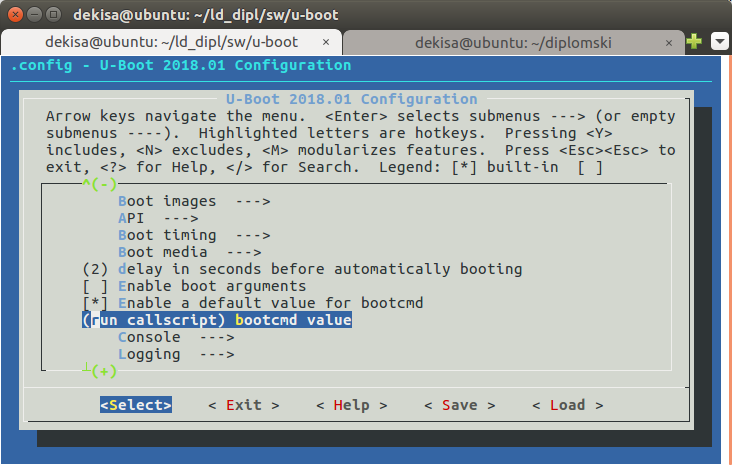
\includegraphics[scale=0.6, trim={0 0 10 60},clip]{img/uboot.png}
\caption{Konfiguracija U-Boot}
\label{slika:uboot}
\end{figure}
\item Izaći iz konfiguracionog menija izborom opcije \texttt{exit} (strelica desno i zatim \texttt{enter}). Sačuvati podešavanja izborom \texttt{Yes}.
\item Otvoriti konfiguracioni \texttt{.h} fajl komandom:\\
\texttt{vi include/configs/socfpga\_de1\_soc.h}
U ovom fajlu je potrebno uneti izmene kao na slici \ref{slika:uboot10}
\begin{figure}[h!]
\centering
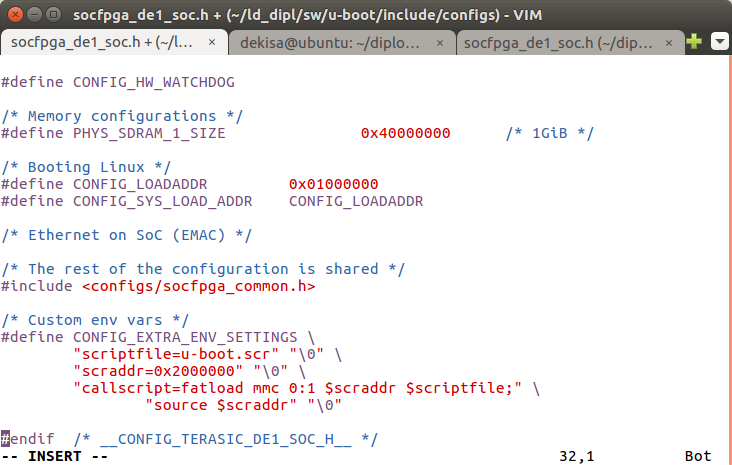
\includegraphics[scale=0.6, trim={0 15 10 60},clip]{img/uboot1.png}
\caption{Izmena U-Boot konfiguracionog fajla}
\label{slika:uboot10}
\end{figure}
\item Pokrenuti kompajliranje U-Boot komandom\\
\texttt{make}
\item Kopirati kompajlirani U-Boot\\
\texttt{cp \textasciitilde/ld\_dipl/sw/u-boot/u-boot.img \textasciitilde/ld\_dipl/sdcard/fat32/u-boot.img }
\item Otvoriti novi tekstualni fajl:\\
\texttt{vi u-boot.script}\\
U ovom fajlu je potrebno napisati skriptu za U-Boot. Ranije u radu je dato objašnjenje skripte, dok se ceo kod nalazi u dodatku rada.
\item Konvertovati napisanu skriptu u odgovarajući format komandom:\\
\texttt{mkimage -A arm -O linux -T script -a 0 -e 0 -n Boot\_script -d u-boot.script u-boot.scr}
\item Kopirati kompajlirani U-Boot\\
\texttt{cp \textasciitilde/ld\_dipl/sw/u-boot/u-boot.scr \textasciitilde/ld\_dipl/sdcard/fat32/u-boot.scr }

\subsubsection{Linuks kernel}
\item Preuzeti izvorni kod Linuks kernela:\\
\texttt{git clone git://github.com/torvalds/linux \textasciitilde/ld\_dipl/sw/linux}
\item Promeniti radni direktorijum\\
\texttt{cd \textasciitilde/ld\_dipl/sw/linux}
\item Napraviti novu granu na osnovu verzije 4.6-rc2 komandom:\\ \texttt{git checkout 4.6-rc2 -b tmp}
\item Konfigurisati linuks za Cyclone V arhitekturu\\
\texttt{make socfpga\_defconfig}
\item Pokrenuti kompajliranje linuksa\\
\texttt{make zImage}
\item Kopirati kompajlirani kernel u pripremni folder\\
\texttt{cp arch/arm/boot/zImage \textasciitilde/ld\_dipl/sdcard/fat32/zImage}


\subsubsection*{Ručno pisanje Device Tree}
\item Početi od Device Tree fajla\\
\texttt{cp arch/arm/boot/dts/socfpga\_cyclone5\_socdk.dts \\arch/arm/boot/dts/socfpga\_cyclone5\_ld\_dipl.dts}
\item Isključiti \texttt{CAN} podešavanjem parametra \texttt{status = 'disabled'}. Ovaj korak je neophodan za uspešno pokretanje sistema jer DE1-SoC nema \texttt{CAN}. Pogledati sliku \ref{slika:dts1}
\item Iz Device Tree fajla generisanog Alterinim alatom izdvojiti samo najbitnije informacije i upisati u novi fajl. Pogledati sliku \ref{slika:dts1}
\begin{figure}[h!]
\centering
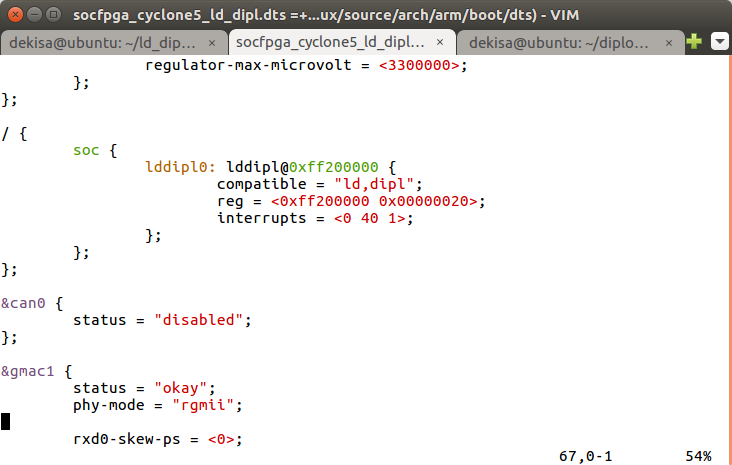
\includegraphics[scale=0.6,trim={0 15 10 60},clip]{img/dts1.png}
\caption{Izmena Device Tree fajla}
\label{slika:uboot1}
\end{figure}
\item Pokrenuti kompajliranje Device Tree fajla\\
\texttt{make socfpga\_cyclone5\_ld\_dipl.dtb}
\item Kopirati kompajlirani Device Tree Blob u pripremni folder\\
\texttt{cp \textasciitilde/ld\_dipl/sw/linux/arch/arm/boot/dts/socfpga\_cyclone5\_ld\_dipl.dtb \\ \textasciitilde/ld\_dipl/sdcard/fat32/socfpga.dtb }


\subsubsection{Kompajliranje drajvera}
\item Promeniti radni folder\\
\texttt{cd \textasciitilde/ld\_dipl/sw/device\_driver}\\
U ovom folderu se nalazi izvorni fajl drajvera \texttt{ld\_dipl.c} i odgovarajući \texttt{Makefile}
\item Podesiti promenljivu koja ukazuje na izvorni kod linuks kernela\\
\texttt{export OUT=\textasciitilde/ld\_dipl/sw/linux}
\item Pokrenuti kompajliranje komandom\\
\texttt{make}
\item Kopirati kompajlirani drajver u pripremni direktorijum\\
\texttt{cp \textasciitilde/ld\_dipl/sw/device\_driver/ld\_dipl.ko \textasciitilde/ld\_dipl/sdcard/ld\_dipl.ko }

\subsubsection{Generisanje Root File System}
\item Preuziti \texttt{Buildroot}
\texttt{git clone git://git.busybox.net/buildroot \textasciitilde/ld\_dipl/sw/buildroot}
\item Promeniti radni folder\\
\texttt{cd \textasciitilde/ld\_dipl/sw/buildroot}
\item Napraviti novu granu na osnovu verzije 2017.08 komandom:
\texttt{git checkout 2017.08 -b tmp}
\item Pokrenuti konfiguracioni meni komandom\\
\texttt{make menuconfig}
\item U konfoguracionim meniju izvršiti sledeće izmene
\begin{enumerate}
\item Target options ---
	\begin{itemize}
	\item Target Architecture (ARM(little endian))
	\item Target Architecture Variant (cortex-A9)
	\item Target ABI (EABIhf)
	\item Floating point strategy (VFPv3)
	\end{itemize}
\item Toolchain ---
	\begin{itemize}
	\item Toolchain type (External toolchain)
	\item Toolchain (Linaro ARM 2017.11)
	\item Toolchain origin (Pre-installed toolchain) ---\\ \texttt{\textasciitilde/ld\_dipl/sw/gcc-linaro-7.2.1-2017.11-x86\_64\_arm-linux-gnueabihf}
	\end{itemize}
\item Kernel ---\
	\begin{itemize}
	\item []Linux Kernel
	\end{itemize}
\end{enumerate}
\item Pokrenuti izvršavanje komandom\\
\texttt{make}
\item Kopirati fajl sistem u pripremni direktorijum\\
\texttt{cp \textasciitilde/ld\_dipl/sw/buildroot/output/images/rootfs.tar \textasciitilde/ld\_dipl/sdcard/rootfs.tar }

\subsubsection{Priprema SD kartice}
\item Ubaciti SD karticu u računar. Zaključiti pod kojim imenom se kartica pojavila u sistemskom folderu \texttt{/dev} (za primer je uzeto \texttt{/dev/sdx} )
\item Formatirati SD karticu komandom\\
\texttt{sudo dd if=/dev/zero of=/dev/sdx bs=512 count=1}
\item Particionisati SD karticu pokretanjem interaktivnog programa \texttt{fdisk}\\
\texttt{ sudo fdisk /dev/sdx}\\
	u kom treba uneti sledeće komande\\
	\texttt{
	n p 3 <default> 4095 t a2 \\
 	n p 1 <default> +32M t 1 b \\
 	n p 2 <default> +512M t 2 83 \\
 	w \\
 	}
\item Napraviti prazne fajl sisteme na odgovarajućim particijama\\
\texttt{sudo mkfs.vfat /dev/sdx1\\
sudo mkfs.ext3 -F /dev/sdx2}
\item Promeniti radni folder\\
\texttt{cd \textasciitilde/ld\_dipl/sdcard}
\item Napraviti foldere na koje će se mount-ovati SD kartica\\
\texttt{
mkdir mountfat32\\
mkdir mountext3
}
\item Mount-ovati odgovarajuće particije\\
\texttt{
sudo mount /dev/sdx1 \textasciitilde/ld\_dipl/sdcard/mountfat32 \\
sudo mount /dev/sdx2 \textasciitilde/ld\_dipl/sdcard/mountext3
}
\item Napisati Preloader na odgovarajuću particiju\\
\texttt{sudo dd if=\textasciitilde/ld\_dipl/sdcard/a2/preloader-mkpimage.bin of=/dev/sdx3 bs=64K seek=0}
\item Kopirati binarne fajlove za pokretanje sistema na odgovarajuću particiju\\
\texttt{sudo cp \textasciitilde/ld\_dipl/sdcard/fat32/* \textasciitilde/ld\_dipl/sdcard/mountfat32} 
\item Otpakovati fajlsistem na SD karticu\\
\texttt{taf -xf rootfs.tar mountext3}
\item Kopirati modul drajvera na SD karticu\\
\texttt{cp ld\_dipl.ko mountext3/root/home}
\item Uveriti se da su svi fajlovi uspešno kopirani komandom\\
\texttt{sync}
\item Unmount-ovati sve particije\\
\texttt{umount \textasciitilde/ld\_dipl/sdcard/mountfat32
umount \textasciitilde/ld\_dipl/sdcard/mountext3}

\subsubsection{Testiranje sistema}
\item Proverti da li su \texttt{MSEL} podešeni za konfigurisanje FPGA sa HSP (ima negde lepa slika)
\item Pruključiti DE1-SoC na napajanje
\item Povezati Mini USB kablom PC računar i port na DE1-SoC ploči koji je obležen sa UART
\item Ubaciti SD karticu u odgovarajući slot
\item Na PC računaru pokrenuti i podseiti \texttt{minicom}\\
\texttt{sudo minicom -s}
\item U podešavanjima \texttt{Serial port setup} uneti izmene kao na slici \ref{slika:minicom} (može se razlikovati ime \texttt{Setial device})
\begin{figure}[h!]
\centering
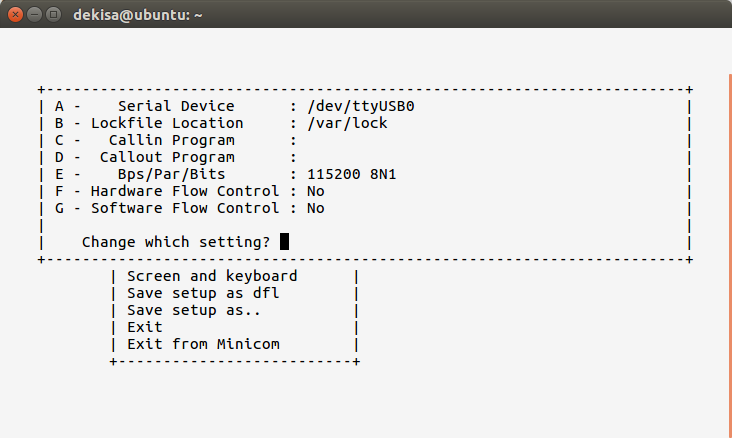
\includegraphics[scale=0.6,trim={0 15 10 60},clip]{img/minicom.png}
\caption{Podešavanje \texttt{minicom}-a}
\label{slika:minicom}
\end{figure}
\item Pokrenuti DE1-SoC pritiskom crvenog tastera
\item Nakon pokretanja sistema potrebno je ulogovati se kao korisnik sa:q\\
\texttt{Username:root\\
Password:root}
\item Učitati modul drajvera u linuks kernel komandom:\\
\texttt{insmod /root/home/ld\_dipl.ko}
\item Promeniti radni direktorijum:\\
\texttt{cd /sys/bus/platform/}
\item Uveriti se da su se pojavili sistemski fajlovi komandom \texttt{ls}
\item Uključiti LE diode upisom u fajl \texttt{leds} i omogućiti pristizanje prekidnog zahteva upisom u fajl \texttt{irq\_mask}
\end{enumerate}